\chapter{Tecnología}

\chapter{Capa de Tecnologia}

\section{Introducción}
En esta capa de aplicaciones observaremos los principales conceptos de comunicación entre componentes por medio de interfaces, donde en los siguientes diagramas se pueden observar los principales comportamientos del aplicativo mediante 4 puntos de vista: Comportamiento de aplicación, Cooperación de aplicación, Estructura de aplicación y el uso de la aplicación.\\
Tal como mencionamos anteriormente, en nuestra capa de aplicación se caracteriza por poseer una arquitectura de componentes, de tal forma que  mostramos las principales funciones dentro de cada componente y ademas como se relacionan y comunican cada uno de estos, de tal forma que observemos como sera el comportamiento y la logica de la aplicación

\section{Punto de Vista de Infraestructura}
\subsection{Descripción}
El punto de vista de infraestructura contiene los elementos de hardware y de software correspondientes a la infraestructura que soporta la capa de aplicación, en este diagrama podemos observar elementos ales como dispositivos físicos, redes o sistemas de software tales como: Bases de datos o sistemas operativos.

\subsubsection{Caso de Estudio}


\begin{figure}[H]
	\centering
	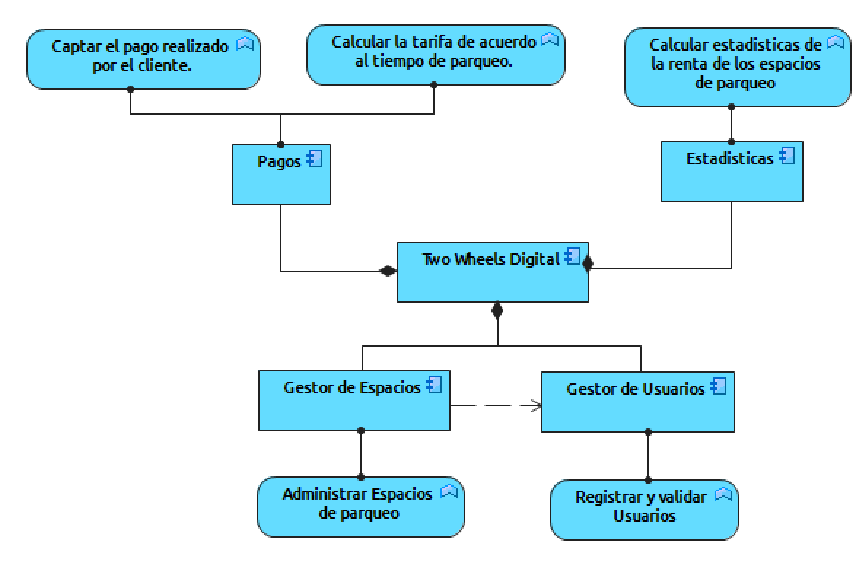
\includegraphics[width=1.0\textwidth]{imagenes/Caso_Estudio/Tecnologia/ComAplicacion.PDF}
	\caption{Caso de estudio: Punto de vista de Infraesructura.}
	\label{fig:gap_analysis}
\end{figure}

\section{Punto de Vista de Uso de Infraestructura}
\subsection{Descripción}
El punto de vista de Uso de Infraestructura muestra como las aplicaciones están soportadas por una infraestructura de hardware y software en la que los servicios de infraestructura  son ofrecidos por los dispositivos mientras que las  redes y los sistemas de software proporcionan las aplicaciones. Este punto de vista juega un papel importante en el análisis del rendimiento y la escalabilidad, ya que relaciona la infraestructura física con el mundo lógico de las aplicaciones. Es muy útil para determinar el rendimiento y los requisitos de calidad en la infraestructura en función de las demandas de las distintas aplicaciones que lo utilizan.

\subsubsection{Metamodelo}
\begin{figure}[H]
	\centering
	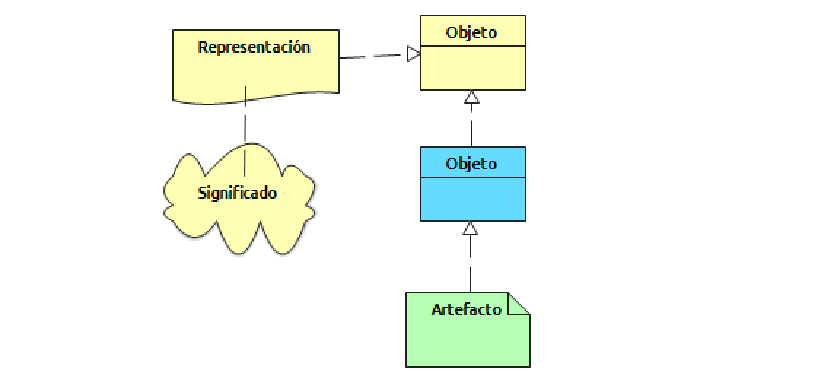
\includegraphics[width=1.0\textwidth]{imagenes/Metamodelos/Tecnologia/Estructura_informacion.PDF}
	\caption{Metamodelo: Punto de Vista de Uso de Infraestrucutra.}
	\label{fig:gap_analysis}
\end{figure}


\subsubsection{Caso de Estudio}


\begin{figure}[H]
	\centering
	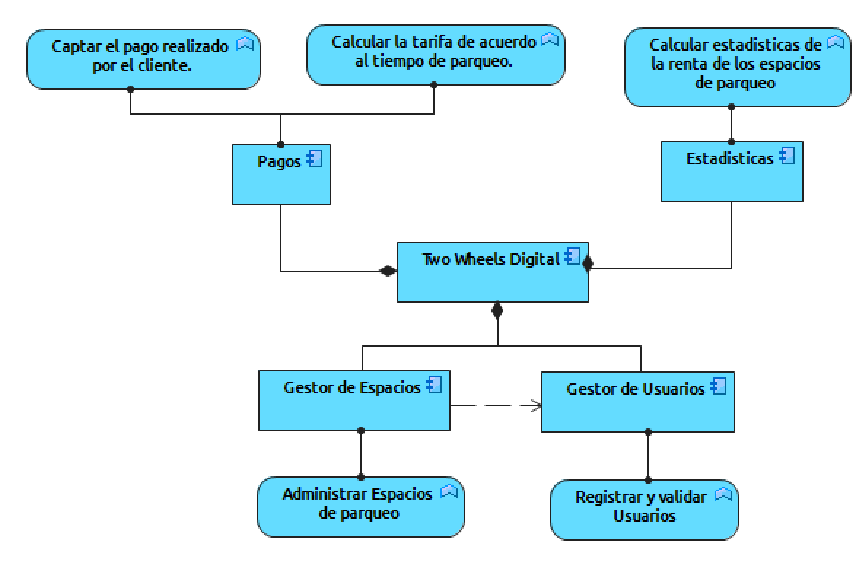
\includegraphics[width=1.0\textwidth]{imagenes/Caso_Estudio/Tecnologia/ComAplicacion.PDF}
	\caption{Caso de estudio: Punto de vista de Uso de Infraesructura.}
	\label{fig:gap_analysis}
\end{figure}


\section{Punto de Vista de Organización e implementación}
\subsection{Descripción}
El punto de vista de organización e implementación muestra como se implementan una o mas aplicaciones o componentes en la insfraestructura. Esto se comprende como el mapeo de aplicaciones lógicas a su respectivos componente o artefacto físico, de igual manera se puede evidenciar un mapeo de  la información que utilizan estas.

\subsubsection{Metamodelo}
\begin{figure}[H]
	\centering
	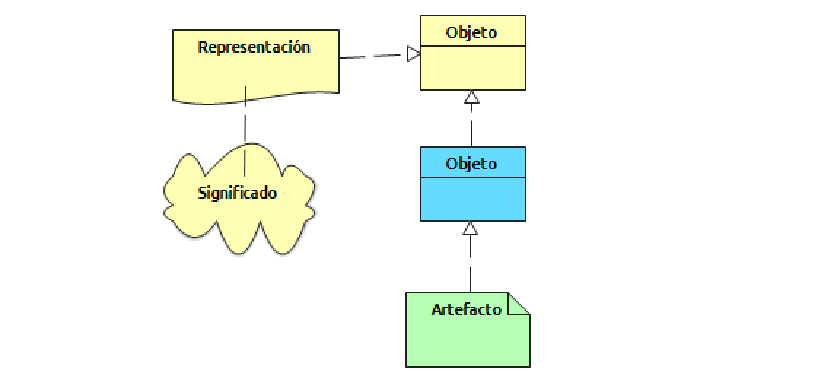
\includegraphics[width=1.0\textwidth]{imagenes/Metamodelos/Tecnologia/Estructura_informacion.PDF}
	\caption{Metamodelo: Punto de Vista de Organización e Implementación.}
	\label{fig:gap_analysis}
\end{figure}

\subsubsection{Caso de Estudio}


\begin{figure}[H]
	\centering
	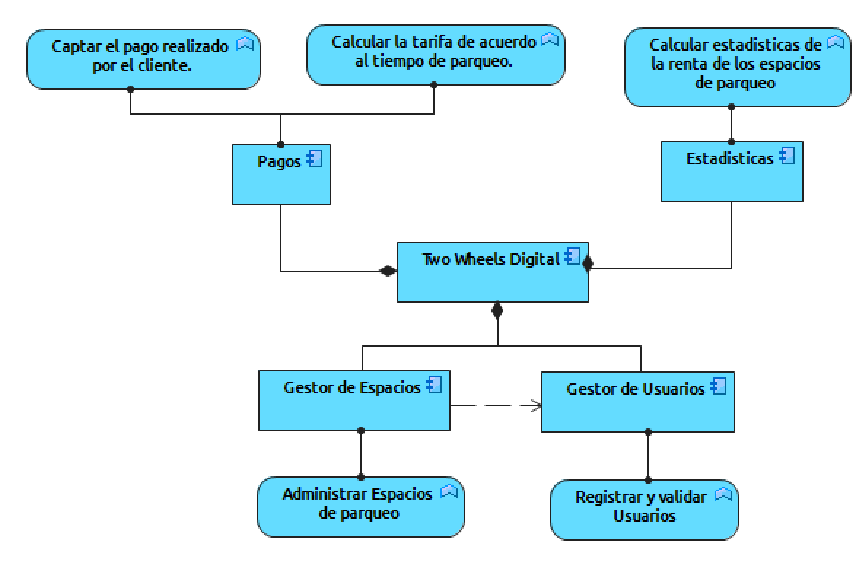
\includegraphics[width=1.0\textwidth]{imagenes/Caso_Estudio/Tecnologia/ComAplicacion.PDF}
	\caption{Caso de estudio: Punto de Vista de Organización e implementación.}
	\label{fig:gap_analysis}
\end{figure}


\section{Punto de Vista de Estructura de Información}
\subsection{Descripción}
El punto de vista de la estructura de información muestra la estructura de la información utilizada en la: empresa, proceso o una aplicación comercial específica; esto en términos de tipos de datos o estructuras de clases (orientadas a objetos). Además, puede mostrar cómo la información se representa en el nivel de negocio, en el nivel de aplicación mediante las estructuras de datos utilizadas allí, y cómo estas se asignan a la infraestructura subyacente mediante artefactos.

\subsubsection{Metamodelo}
\begin{figure}[H]
	\centering
	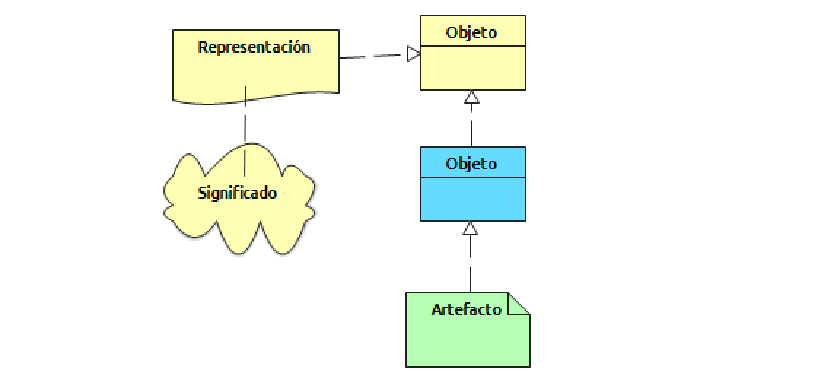
\includegraphics[width=1.0\textwidth]{imagenes/Metamodelos/Tecnologia/Estructura_informacion.PDF}
	\caption{Metamodelo: Punto de Vista de Estructura de Información.}
	\label{fig:gap_analysis}
\end{figure}

\subsubsection{Caso de Estudio}


\begin{figure}[H]
	\centering
	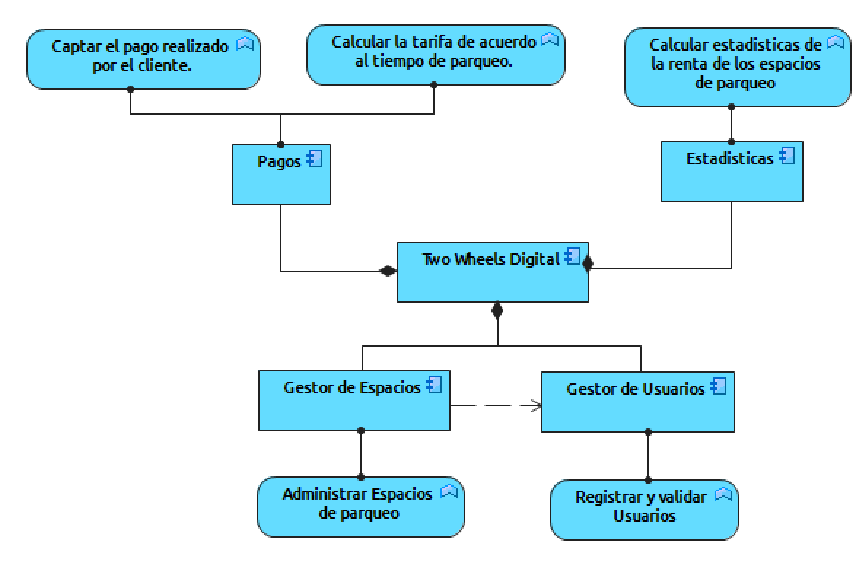
\includegraphics[width=1.0\textwidth]{imagenes/Caso_Estudio/Tecnologia/ComAplicacion.PDF}
	\caption{Caso de estudio: Punto de Vista de Estructura de información.}
	\label{fig:gap_analysis}
\end{figure}


\section{Punto de Vista de Realización del Servicio}
\subsection{Descripción}
El punto de vista de Realización del servicio se utiliza para mostrar cómo uno o más servicios de negocio se realizan mediante los procesos subyacentes (y, en ocasiones, mediante los componentes de la aplicación). Por lo tanto, forma el puente entre el punto de vista del producto y la vista del proceso de negocios. Proporciona una "vista desde el exterior" en uno o más procesos comerciales.

\subsubsection{Metamodelo}
\begin{figure}[H]
	\centering
	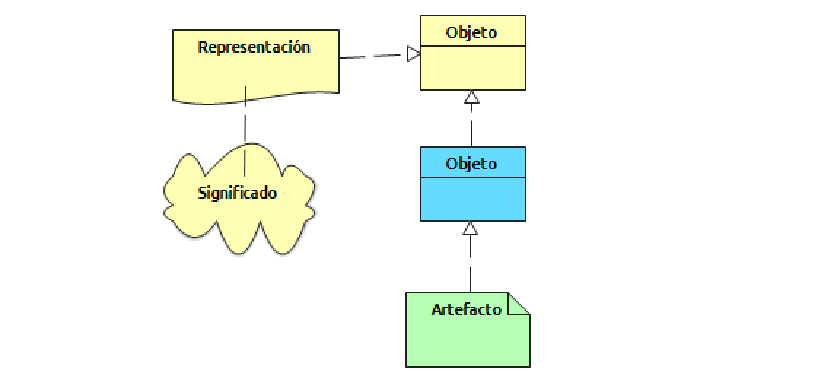
\includegraphics[width=1.0\textwidth]{imagenes/Metamodelos/Tecnologia/Estructura_informacion.PDF}
	\caption{Metamodelo: Punto de Vista de Realización del Servicio.}
	\label{fig:gap_analysis}
\end{figure}

\subsubsection{Caso de Estudio}

\begin{figure}[H]
	\centering
	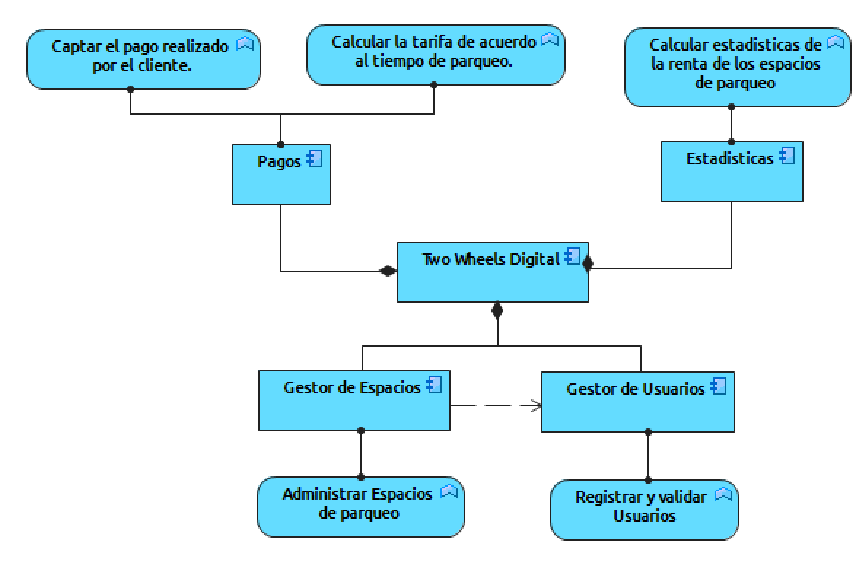
\includegraphics[width=1.0\textwidth]{imagenes/Caso_Estudio/Tecnologia/ComAplicacion.PDF}
	\caption{Caso de estudio: Punto de Vista de Realizacion del Servicio.}
	\label{fig:gap_analysis}
\end{figure}


\section{Punto de Vista de Capas}
\subsection{Descripción}
El punto de vista en capas representa varias capas y aspectos de una arquitectura empresarial en un diagrama. El principio estructural detrás de un punto de vista completamente estratificado es que cada capa dedicada expone, mediante la relación de "realización", una capa de servicios, que luego son "utilizados por" la siguiente capa dedicada. Por lo tanto, podemos separar fácilmente la estructura interna y la organización de una capa dedicada de su comportamiento externo observable expresado como la capa de servicio que la capa dedicada realiza.  El objetivo principal del punto de vista de capas es proporcionar información general en un diagrama.

\subsubsection{Metamodelo}
\begin{figure}[H]
	\centering
	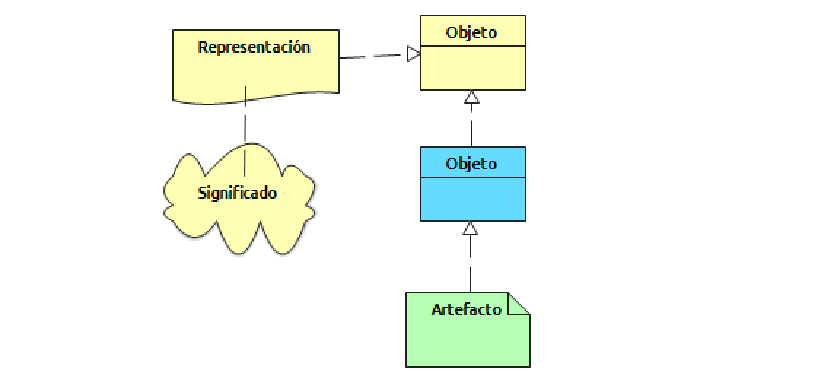
\includegraphics[width=1.0\textwidth]{imagenes/Metamodelos/Tecnologia/Estructura_informacion.PDF}
	\caption{Metamodelo: Punto de Vista de Uso de capas.}
	\label{fig:gap_analysis}
\end{figure}

\subsubsection{Caso de Estudio}


\begin{figure}[H]
	\centering
	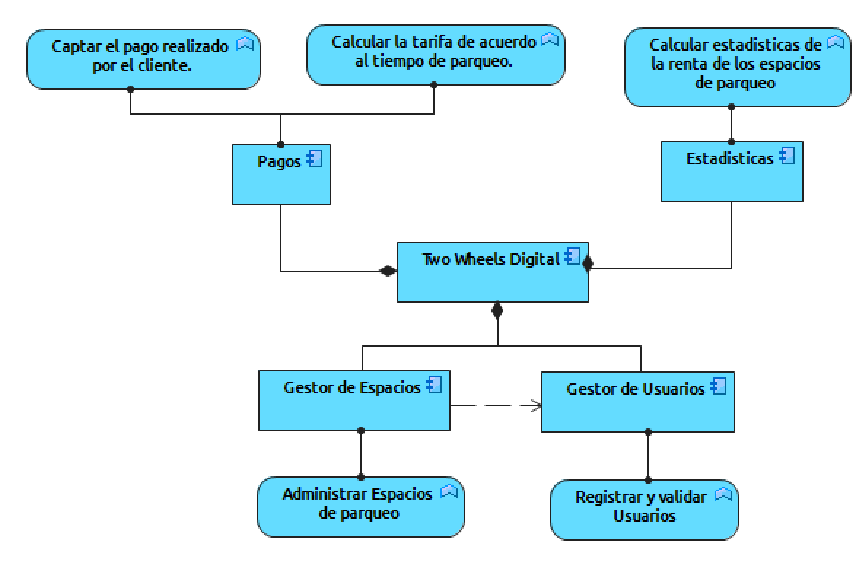
\includegraphics[width=1.0\textwidth]{imagenes/Caso_Estudio/Tecnologia/ComAplicacion.PDF}
	\caption{Caso de estudio: Punto de Vista de Capas.}
	\label{fig:gap_analysis}
\end{figure}

